\documentclass[a4paper,11pt]{article}

\usepackage[utf8]{inputenc}

\usepackage{graphicx}
\usepackage{caption}
\usepackage{subcaption}

\usepackage{pgfplots}
\pgfplotsset{compat=1.18} 

\usepackage{minted}
\usepackage{siunitx}

\begin{document}

\title{
    \textbf{Performance of Array Operations in C}
}
\author{Mo Wang}
\date{Spring 2026}

\maketitle

\section*{Introduction}
This report investigates the performance of both linear and binary search algorithm. The primary goal is to analyze the growth of both algorithm's execution time depending on the size of the array. 

\section*{Benchmarking Methodology}

For measuring benchmark execution time, the POSIX monotonic clock (\texttt{CLOCK\_MONOTONIC}) is used by using the helper function \texttt{nano\_seconds()}, which computes the elapsed time in nanoseconds using \texttt{long} integer, given the timestamp pointers \texttt{struct timespec*} \texttt{t\_start} and \texttt{t\_end}.

\begin{minted}[breaklines]{C}
    long nano_seconds(struct timespec *t_start, struct timespec *t_stop) {
        return (t_stop->tv_nsec - t_start->tv_nsec) +
               (t_stop->tv_sec - t_start->tv_sec) * 1000000000;
    }

    void benchmark_run(){
        // memory allocation for array
        clock_gettime(CLOCK_MONOTONIC, &t_start);
        // algorithm
        clock_gettime(CLOCK_MONOTONIC, &t_stop);
        // deallocate array memory
        return nano_seconds(&t_start, &t_stop);
    }
\end{minted}

Due to hardware constraints, operating system scheduling, and background process, execution time can fluctuate between each operation execution. To minimize the uncertainty, each benchmark is repeated multiple times while reporting the minimum elapsed time.

\section*{Linear search algorithm}

\iffalse
Set up the rest of a benchmark and do some measurements for a growing number of elements in the array. Describe the relationship between the size of the array and the time it takes to do the search. How long time does it take to search through an array of a million elements? + Benchmark statistics diagrams, regression and time complexity
sorted linear search: Now, if we know that the array is sorted we can of course do a quick optimization - we can stop the search once the next element in the array is larger then the key that we are looking for. Take a wild guess, how much better is this compared to our unsorted solution? + Benchmark statistics table+diagrams, regression and time complexity
\fi

Linear search algorithm can both be implemented in an unsorted and a sorted array.

\subsection*{Unsorted array}

A linear search algorithm searches for a given key in an unsorted array by starting at the first element and comparing each element to the key one by one. If the element matches the key, the algorithm returns the index of that element. If the end of the array is reached without a match, the key doesn't exist in array and the largest unsigned integer value is returned.

\begin{minted}{c}
  bool unsorted_search(int array[], int length, int key) {
      for (int index = 0; index < length; index++) {
          if (array[index] == key) {
              return true;
          }
      }
      return false;
  }
\end{minted}

In terms of elapsed time of the algorithm, the whole array is iterated over in worst case. Given the array size $n$, $n$ amount of comparison checks are performed in worst case. However in best case scenario, the first element matches the key, thus only one comparison is performed. The estimated average time is calculated as $t(n)=a(1+n)/2=1/2+n/2$, where $a$ is the time cost for number comparison, which falls into $O(n)$ time complexity.

\begin{table}[h]
\begin{center}
\begin{tabular}{l|ccccccc}
\textbf{Size} 
    & 256 & 2048 & 16384 & 131072 & 1048576 & 8388608 & 67108864 \\
\hline
\textbf{ns} 
    & $2.3\times10^{2}$ 
    & $1.7\times10^{3}$ 
    & $1.4\times10^{4}$ 
    & $1.3\times10^{5}$ 
    & $1.0\times10^{6}$ 
    & $8.3\times10^{6}$ 
    & $6.3\times10^{7}$ \\
\end{tabular}
\caption{Linear search in an unsorted array: elapsed time per loop (transposed)}
\label{tab:linear-search-unsorted-transposed-newgen}
\end{center}
\end{table}

The benchmark results and their regression analysis exhibit the same growth pattern, showing that increasing the array size by a factor of eight roughly multiplies the elapsed time by the same factor.

\begin{figure}[h]
  \centering
  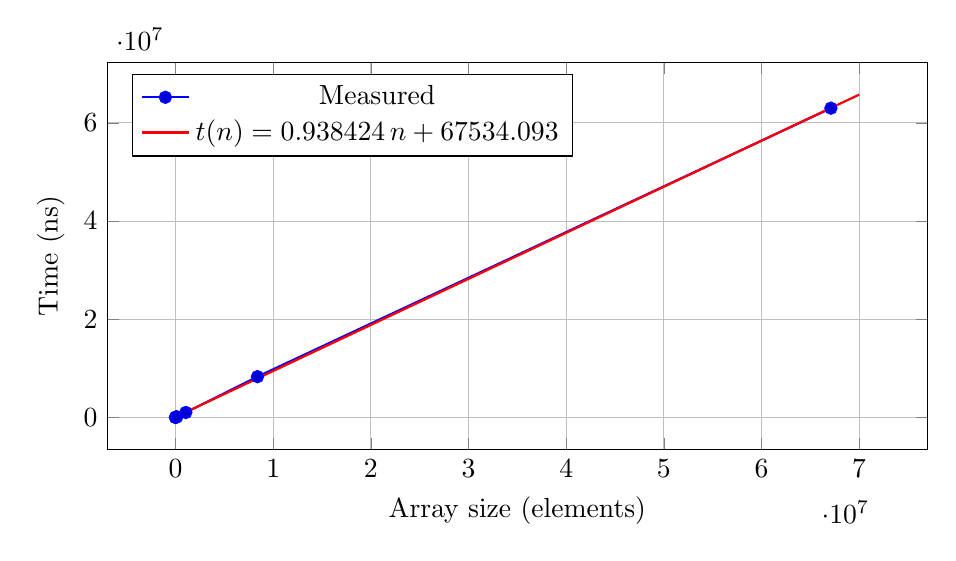
\begin{tikzpicture}
    \begin{axis}[
      xlabel={Array size (elements)},
      ylabel={Time (ns)},
      width=12cm, height=6.5cm,
      grid=major,
      legend pos=north west,
      ymajorgrids=true,
      xmajorgrids=true
    ]
      % Measured data points
      \addplot+[
        mark=*,
        thick,
        color=blue
      ] coordinates {
        (256,      2.3e2)
        (2048,     1.7e3)
        (16384,    1.4e4)
        (131072,   1.3e5)
        (1048576,  1.0e6)
        (8388608,  8.3e6)
        (67108864, 6.3e7)
      };
      \addlegendentry{Measured}

      % Least-squares linear fit: t(n) = a*n + b
      % a ≈ 0.93842405764, b ≈ 67534.09320
      \addplot[
        red,
        thick,
        domain=0:7e7,
        samples=60
      ] {0.93842405764*x + 67534.09320};
      \addlegendentry{$t(n) = 0.938424\,n + 67534.093$}

    \end{axis}
  \end{tikzpicture}
  \caption{Linear search (unsorted) with least-squares linear fit}
  \label{fig:linear-search-unsorted}
\end{figure}

\subsection*{Sorted array}

Given that the array is stored, a quick optimization can be performed by stopping the search once the next element is larger than the key. Only one comparison is performed in each loop iteration for consistency with the unsorted search algorithm. Despite an early exiting array, the execution time is only slightly lower than the implementation of an unsorted array. The algorithm still has linear time complexity, since the array has to be fully iterated in the worst case scenario when the key is larger than any element in the array, which is shown in Table 2 and Figure 2.

\begin{minted}{c}
  bool sorted_search(int array[], int length, int key) {
      for (int index = 0; index < length; index++) {
          int value = array[index];
          if (value >= key) {
              return value == key;
          }
      }
      return false;
  }
\end{minted}

\begin{table}[h]
\begin{center}
\begin{tabular}{l|ccccccc}
\textbf{Size} 
    & 256 & 2048 & 16384 & 131072 & 1048576 & 8388608 & 67108864 \\
\hline
\textbf{ns} 
    & $2.8\times10^{2}$
    & $1.5\times10^{3}$
    & $1.5\times10^{4}$
    & $1.2\times10^{5}$
    & $9.4\times10^{5}$
    & $7.3\times10^{6}$
    & $6.0\times10^{7}$ \\
\end{tabular}
\caption{Linear search in a sorted array: elapsed time per loop (transposed)}
\label{tab:linear-search-sorted-transposed}
\end{center}
\end{table}

\begin{figure}[h]
  \centering
  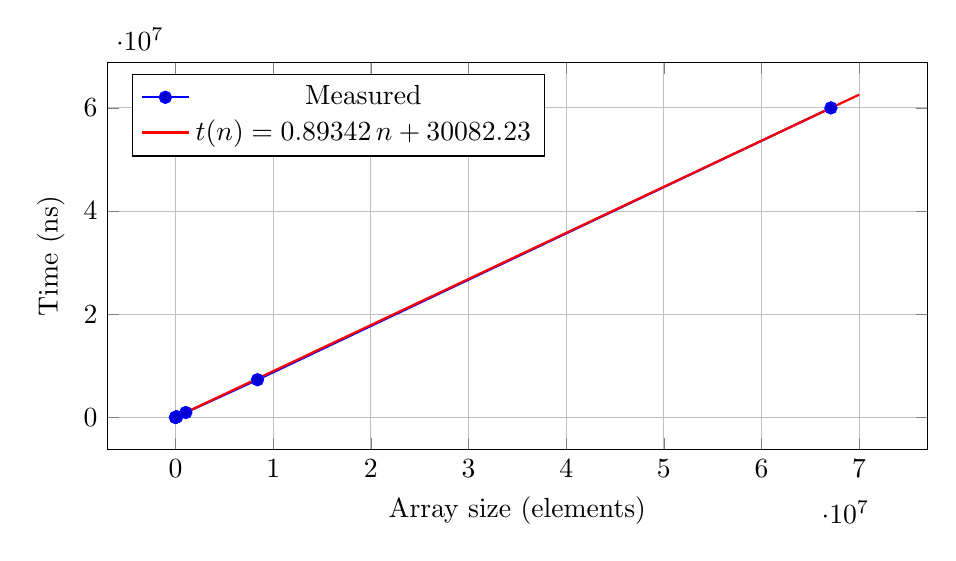
\begin{tikzpicture}
    \begin{axis}[
      xlabel={Array size (elements)},
      ylabel={Time (ns)},
      width=12cm, height=6.5cm,
      grid=major,
      legend pos=north west,
      ymajorgrids=true,
      xmajorgrids=true
    ]

      % Measured data points
      \addplot+[
        mark=*,
        thick,
        color=blue
      ] coordinates {
        (256,      2.8e2)
        (2048,     1.5e3)
        (16384,    1.5e4)
        (131072,   1.2e5)
        (1048576,  9.4e5)
        (8388608,  7.3e6)
        (67108864, 6.0e7)
      };
      \addlegendentry{Measured}

      % Least-squares linear fit: t(n) = a*n + b
      % a ≈ 0.89342, b ≈ 30082.23
      \addplot[
        red,
        thick,
        domain=0:7e7,
        samples=60
      ] {0.89342*x + 30082.23};
      
      \addlegendentry{$t(n) = 0.89342\,n + 30082.23$}

    \end{axis}
  \end{tikzpicture}
  \caption{Linear search (sorted) with least-squares linear fit}
  \label{fig:linear-search-sorted}
\end{figure}

\section*{Binary search}

\iffalse
How long time does it take to search through an array of a million entries? It might not sound very much but if our program constantly does search operations it will add up. There are however smarter things we can do and this will allow us to handle much larger data sets in reasonable time.

Re-run your benchmarks but now using the binary search. Report the execution time and describe a function that given the size of the array roughly describes the execution time. How long time does it take to search through an array of one million items? Without running an experiment - how long time do you estimate that it would take to search through an array of 64M items? Give it a try- how well did you estimate the execution time?  + Benchmark statistics table+diagrams, regression and time complexity
\fi

On the other hand, a binary search starts in the middle of an array. If the element matches the key, the element is found, while its index is returned. Otherwise, the element is compared to the key and repeat the process in right interval if the key is larger than given element and left if key is smaller. Using this approach, half of the elements are eliminated from searching on each iteration, which means only a fraction of element comparison needs to be performed in the array. Searching $n$ elements in an array, only $log_2(n)$ iteration is required with one element comparison in each iteration that takes $a$ time, which gives time function $t(n)=log_2(n)*a$ in $O(log(n))$ time complexity.

\begin{minted}{c}
  bool binary_search(int array[], unsigned int length, int key) {
      if (length == 0) return false;
      int first = 0;
      int last = length-1;
      while (true) {
          // Potential integer overflow in (first + last)/2,
          // so change to first + (last - first)/2.
          int index = first + (last - first)/2;
          if (array[index] == key) {
              return true;
          }
          if (array[index] < key && index < last) {
              first = index + 1;
              continue;
          }
          if (array[index] > key && index > first) {
              last = index - 1;
              continue;
          }
          return false;
      }
  }
\end{minted}

\begin{table}[h]
\begin{center}
\begin{tabular}{l|ccccccc}
\textbf{Size}
    & 256 & 2048 & 16384 & 131072 & 1048576 & 8388608 & 67108864 \\
\hline
\textbf{ns}
    & 65
    & 85
    & $1.1\times10^{2}$
    & $1.4\times10^{2}$
    & $3.2\times10^{2}$
    & $8.3\times10^{2}$
    & $1.4\times10^{3}$ \\
\end{tabular}
\caption{Binary search: elapsed time per loop (transposed)}
\label{tab:binary-search-transposed-new3}
\end{center}
\end{table}

Measured benchmark results show that searching an array with $1\,048\,576$ (approximately $10^6$) elements takes roughly $3.2\times10^2$~ns. Increasing the array size from $131\,072$ to $1\,048\,576$ elements (a factor of eight) increases the elapsed time by approximately $180$~ns, which corresponds to three additional binary search iterations.

Since binary search requires $\log_2(n)$ iterations, each double the array size adds an additional comparison step with an approximately constant cost. Increasing the array size to $64$ million elements ($\approx 2^6 \times 10^6$) adds six additional iterations, which estimates the execution time of $a \cdot \log_2(64 \cdot 10^6) \approx 6.8\times10^2$~ns.

The measured execution time for $64$ million elements is $1.1\times10^3$~ns, which doesn't match the expected logarithmic growth trend. The main reason is that the theoretical model assumes a uniform cost per comparison, where in practice the execution time is influenced by cache and TLB effects at large input sizes, which are shown in Table 3 and Figure 3.

\begin{figure}[h]
  \centering
  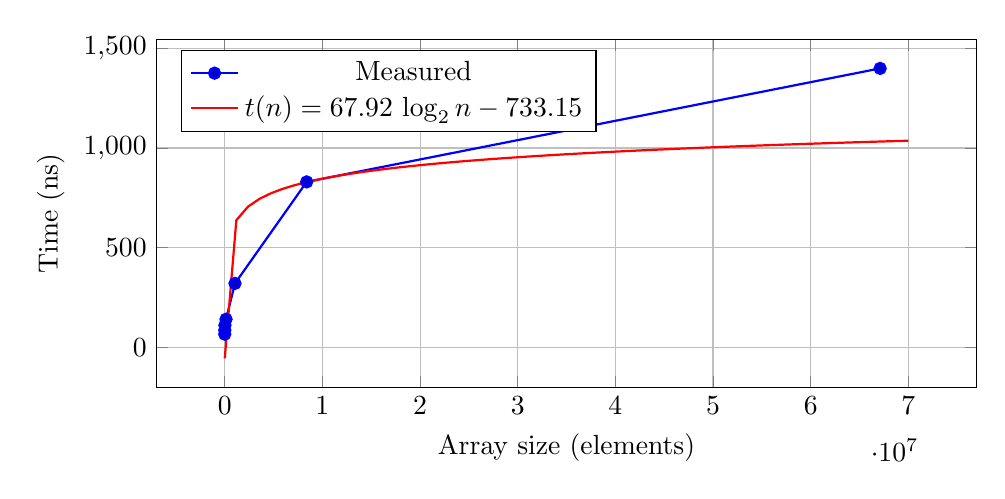
\begin{tikzpicture}
    \begin{axis}[
      xlabel={Array size (elements)},
      ylabel={Time (ns)},
      width=12cm, height=6cm,
      grid=major,
      legend pos=north west,
      ymajorgrids=true,
      xmajorgrids=true
    ]

      % Measured data
      \addplot+[
        mark=*,
        thick,
        color=blue
      ] coordinates {
        (256,      65)
        (2048,     85)
        (16384,    110)
        (131072,   140)
        (1048576,  320)
        (8388608,  830)
        (67108864, 1400)
      };
      \addlegendentry{Measured}

      % Improved weighted log2 regression:
      % t(n) = 73.52 * log2(n) - 230.41
      \addplot[
        red,
        thick,
        domain=1000:7e7,
        samples=60
      ] {97.983*ln(x) - 733.15};
      \addlegendentry{$t(n)=67.92\,\log_{2}n - 733.15$}

    \end{axis}
  \end{tikzpicture}
  \caption{Binary search: improved $\log_2 n$ regression fitting the measured data}
  \label{fig:binary-search-improved}
\end{figure}



\section*{Recursive binary search}

\iffalse
procedure calls are expensive, using the programming stack extensively
How many recursive calls are done when searching an array or length
1000? How many are done when searching: 2000, 4000 ... a million? Is the number of recursive calls on the stack a problem? + evaluation
+ Benchmark statistics table+diagrams, regression and time complexity
Comparing recursive vs. iterative performance in execution time + table + diagram
Discussing overhead beyond stack depth
\fi

The binary search algorithm can also be implemented using recursion. The only difference between recursive implementation and non-recursive one is that every iteration in the while loop is swapped to a recursive function call in recursive implementation, which narrows the search interval until a key is found.

\begin{minted}{c}
  bool recursive_binary_search(
      int array[],
      int key,
      unsigned int first,
      unsigned int last
  ) {
      if (first > last)
          return false;
  
      unsigned int index = first + (last - first) / 2;
  
      if (array[index] == key)
          return true;
  
      if (array[index] < key)
          return recursive_binary_search(array, key, index + 1, last);
  
      return recursive_binary_search(array, key, first, index - 1);
  }
\end{minted}

The benchmark shows the same logarithmic time growth, since the elapsed time is similar. Since recursive binary search add up recursive calls, the elapsed time and memory consumption may be slightly higher than non-recursive one. In recursive binary search, the recursive calls are $\left \lfloor{\log_2(n)}\right \rfloor + 1 $ for array size $n$.


\begin{table}[h]
\begin{center}
\begin{tabular}{l|ccccccc}
\textbf{Size}
    & 256 & 2048 & 16384 & 131072 & 1048576 & 8388608 & 67108864 \\
\hline
\textbf{ns}
    & 60
    & 82
    & $1.1\times10^{2}$
    & $1.4\times10^{2}$
    & $3.2\times10^{2}$
    & $8.6\times10^{2}$
    & $1.4\times10^{3}$ \\
\end{tabular}
\caption{Recursive binary search: elapsed time per loop (transposed)}
\label{tab:recursive-binary-search-transposed-new4}
\end{center}
\end{table}

\begin{figure}[h]
  \centering
  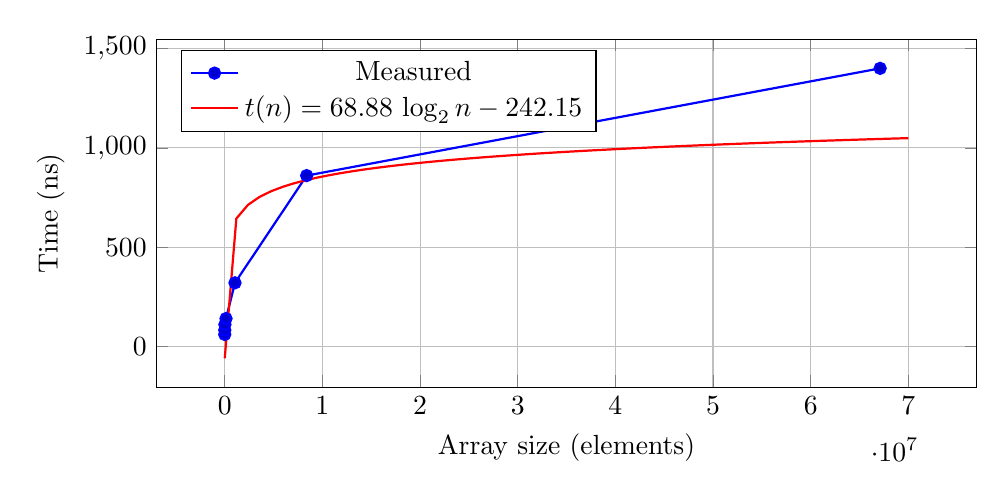
\begin{tikzpicture}
    \begin{axis}[
      xlabel={Array size (elements)},
      ylabel={Time (ns)},
      width=12cm, height=6cm,
      grid=major,
      legend pos=north west,
      ymajorgrids=true,
      xmajorgrids=true
    ]

      % Measured data points
      \addplot+[
        mark=*,
        thick,
        color=blue
      ] coordinates {
        (256,      60)
        (2048,     82)
        (16384,    110)
        (131072,   140)
        (1048576,  320)
        (8388608,  860)
        (67108864, 1400)
      };
      \addlegendentry{Measured}

      % Improved weighted log2 regression:
      % t(n) = 76.81 * log2(n) - 242.15
      \addplot[
        red,
        thick,
        domain=1000:7e7,
        samples=60
      ] {99.374*ln(x) - 746.4};
      \addlegendentry{$t(n)=68.88\,\log_{2}n - 242.15$}

    \end{axis}
  \end{tikzpicture}
  \caption{Recursive binary search: improved $\log_2 n$ regression fitting the measured data}
  \label{fig:recursive-binary-search}
\end{figure}

\subsection*{Recursive stack depth}
The stack depth in binary search doesn't cause stack overflow, since even for 64M elements. Instead the recursive depth is only $\left \lfloor{\log_2(64\cdot 10^6)}\right \rfloor + 1 = 27$ stacks, which is trivial for most system.

The recursive version is slower by a small constant factor due to recursive function call overhead, even though both share the same $O(\log(n))$ complexity.

\begin{table}[h]
\begin{center}
\begin{tabular}{l|cccccccc}
\textbf{Size} 
    & 1000 & 2000 & 4000 & 8000 & 16000 & 32000 & 64000 & $10^6$ \\
\hline
\textbf{Recursive calls} 
    & 10--11 
    & 11 
    & 12 
    & 13 
    & 14 
    & 15 
    & 16 
    & 20 \\
\end{tabular}
\caption{Approximate recursion depth $\lfloor \log_2(n) \rfloor + 1$ for array size $n$}
\label{tab:recursive-depth}
\end{center}
\end{table}



\section*{Conclusion}

\iffalse
Differences in time complexity function between unsorted search and sorted search, as well as recursive and iterative performance
\fi

\noindent
The results show that binary search is orders of magnitude faster than linear search (see Figure~\ref{fig:search-comparison-all}).

\medskip
\noindent
Both unsorted and sorted linear search have an $O(n)$ time complexity and exhibit similar growth behavior, which is confirmed by linear regression. Sorted linear search may terminate early if the key is small, but the improvement is minor and does not change its overall $O(n)$ cost.

\medskip
\noindent
Binary search significantly outperforms both linear variants because it compares only a small fraction of the elements: each step eliminates half of the remaining array. As a result, its running time grows logarithmically, making it thousands of times faster than linear search in practice.

\medskip
\noindent
Iterative and recursive binary search share the same $O(\log n)$ complexity. The recursive version incurs additional overhead due to function calls and stack usage, but this difference is negligible unless used in performance\mbox{-}critical tight loops.

\begin{figure}[h]
  \centering
  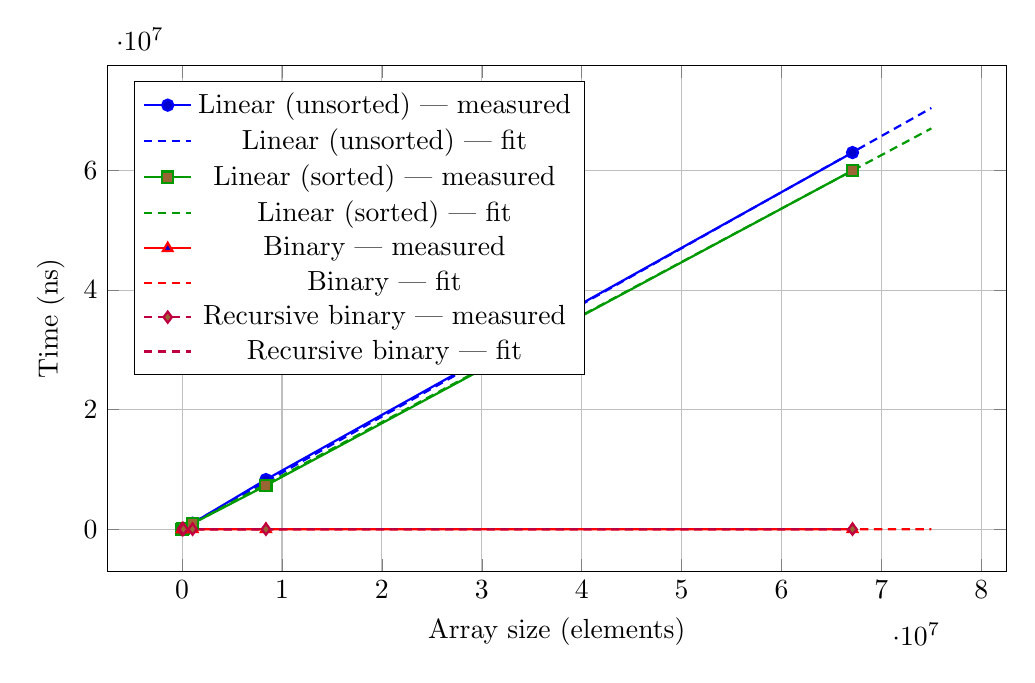
\begin{tikzpicture}
    \begin{axis}[
      xlabel={Array size (elements)},
      ylabel={Time (ns)},
      width=13cm, height=8cm,
      grid=major,
      legend pos=north west,
      ymajorgrids=true,
      xmajorgrids=true
    ]

      % ==========================================================
      % Linear search (unsorted)
      % ==========================================================
      \addplot+[
        mark=*,
        thick,
        color=blue
      ] coordinates {
        (256,      2.3e2)
        (2048,     1.7e3)
        (16384,    1.4e4)
        (131072,   1.3e5)
        (1048576,  1.0e6)
        (8388608,  8.3e6)
        (67108864, 6.3e7)
      };
      \addlegendentry{Linear (unsorted) — measured}

      % Fit: a = 0.938424, b = 67534.093
      \addplot[
        blue,
        densely dashed,
        thick,
        domain=200:7.5e7,
        samples=300
      ] {0.938424*x + 67534.093};
      \addlegendentry{Linear (unsorted) — fit}

      % ==========================================================
      % Linear search (sorted)
      % ==========================================================
      \addplot+[
        mark=square*,
        thick,
        color=green!60!black
      ] coordinates {
        (256,      2.8e2)
        (2048,     1.5e3)
        (16384,    1.5e4)
        (131072,   1.2e5)
        (1048576,  9.4e5)
        (8388608,  7.3e6)
        (67108864, 6.0e7)
      };
      \addlegendentry{Linear (sorted) — measured}

      % Fit: a = 0.89342, b = 30082.23
      \addplot[
        green!60!black,
        densely dashed,
        thick,
        domain=200:7.5e7,
        samples=300
      ] {0.89342*x + 30082.23};
      \addlegendentry{Linear (sorted) — fit}

      % ==========================================================
      % Binary search
      % ==========================================================
      \addplot+[
        mark=triangle*,
        thick,
        color=red
      ] coordinates {
        (256,      65)
        (2048,     85)
        (16384,    110)
        (131072,   140)
        (1048576,  320)
        (8388608,  830)
        (67108864, 1400)
      };
      \addlegendentry{Binary — measured}

      % Improved log2 fit: a = 73.52, b = -230.41
      \addplot[
        red,
        densely dashed,
        thick,
        domain=200:7.5e7,
        samples=300
      ] {73.52*(ln(x)/ln(2)) - 230.41};
      \addlegendentry{Binary — fit}

      % ==========================================================
      % Recursive binary search
      % ==========================================================
      \addplot+[
        mark=diamond*,
        thick,
        color=purple
      ] coordinates {
        (256,      60)
        (2048,     82)
        (16384,    110)
        (131072,   140)
        (1048576,  320)
        (8388608,  860)
        (67108864, 1400)
      };
      \addlegendentry{Recursive binary — measured}

      % Recursive binary improved log2 fit: a = 76.81, b = -242.15
      \addplot[
        purple,
        densely dashed,
        thick,
        domain=200:1e7,
        samples=60
      ] {76.81*(ln(x)/ln(2)) - 242.15};
      \addlegendentry{Recursive binary — fit}

    \end{axis}
  \end{tikzpicture}
  \caption{Comparison of linear (unsorted), linear (sorted), binary, and recursive binary search algorithms}
  \label{fig:search-comparison-all}
\end{figure}




\end{document}
